\documentclass[reqno, fleqn, paper=a4, fontsize=12pt, DIV=11, BCOR=10mm, twoside, titlepage, open=right, bibliography=totoc, numbers=noendperiod, captions=tableheading, headings=normal, parskip]{scrbook} %{scrreprt}
%\documentclass[reqno, fleqn, paper=a4, fontsize=12pt, DIV=11, BCOR=0mm, twoside=semi, titlepage, open=right, bibliography=totoc, numbers=noendperiod, captions=tableheading, headings=normal, parskip]{scrbook} %{scrreprt}
\usepackage{99_style/style_en}
%\usepackage{99_style/styleMarkus}
\color{black}
\usepackage{lmodern}

\graphicspath{{97_graphics/}}
\newcommand*{\GraphicPath}{./97_graphics}%

\usepackage{pgfplots}
\pgfplotsset{compat=1.18}
\usepackage{array}
\usepackage{longtable}
\usepackage{multicol}
\usepackage{ragged2e}
\usepackage{verbatim}
\usepackage{caption}
\usepackage{colortbl}
\usepackage{hhline}
\usepackage{subcaption}
\usepackage[nameinlink]{cleveref}
\usepackage{graphicx}
\usepackage{float}
\usepackage[printonlyused]{acronym} % list of acronyms
\usepackage{algorithmic}
% \usepackage{algorithm}
\numberwithin{algocf}{chapter}
\renewcommand{\thealgocf}{\thechapter.\arabic{algocf}}
\SetAlCapSkip{2ex}
\usepackage{enumitem}
\usepackage{multirow}
\usepackage{booktabs}
\usepackage{siunitx}
\setbool{@fleqn}{false} % equations shall be centered
\newcolumntype{K}[1]{>{\centering\arraybackslash}m{#1}}
\newcolumntype{P}[1]{>{\RaggedRight\hspace{0pt}}p{#1}}
\newcolumntype{P}[1]{>{\centering\arraybackslash}p{#1}}
\newcolumntype{M}[1]{>{\centering\arraybackslash}m{#1}}
\begin{document}
\pagenumbering{roman}
	
\newcommand{\Organization}{FZI - Forschungszentrum Informatik}
\newcommand{\Department}{Embedded Systems and Sensors Engineering}
\newcommand{\Prof}{Prof. Dr.-Ing. Eric Sax} 
\newcommand{\mytitle}{Titel}
\newcommand{\Worktype}{Bachelor / Master Thesis}
\newcommand{\Verfasser}{(B.Sc.) / (M.Sc.) Max Mustermann}
\newcommand{\StartDatum}{TT.MM.JJJJ}
\newcommand{\EndDatum}{TT.MM.JJJJ}
\newcommand{\Betreuer}{Dipl.-Ing./M.Sc.  Max Mustermann}


\renewcommand{\maketitle}{\pagestyle{empty}\begin{titlepage}
\begin{tikzpicture}[overlay]
\node [anchor=north ] at (8,0.5) {%

\includegraphics[width=.13\textwidth]{00_intro/fzi-logo_transparenz.png}
};
\node  at (8,-13) {%
\begin{minipage}{1.1\textwidth}
	\centering \Large \sffamily \textbf{%
		\Organization\\
	}
	\centering \large \sffamily{
		\Department\\
	}	
	\vspace{3cm}
	\centering \LARGE \sffamily \textbf{
		\mytitle\\
	}
	\vspace{2.5cm}
	\centering \Large \sffamily \textbf{
		\Worktype\\
	}
	\vspace{1.5cm}
	\centering \large \sffamily {
		\iflanguage{english}
			{presented by\\}
			{vorgelegt von\\}
			\vspace{0.25cm}
		\Verfasser\\
	}
	\vspace{2.5cm}
	\centering \normalsize  \sffamily {
	\begin{tabular}{@{}ll@{}}
		\iflanguage{english}
			{
				Date: & \qquad \EndDatum\\
				Advisor: & \qquad \Prof\\
				Preceptor: & \qquad \Betreuer\\
			}
			{
				Datum: & \qquad \EndDatum\\
				Referent: & \qquad \Prof\\
				Betreuer: & \qquad \Betreuer\\
			}
	\end{tabular}
	}
\end{minipage}
};
\end{tikzpicture}
\end{titlepage}

\begin{titlepage}
	\vspace*{\fill}
	{\Large\textbf{Declaration}\par}\bigskip%
	I hereby declare that I wrote my Master's Thesis on my own and that I have followed the regulations relating to good scientific practice of the Karlsruhe Institute of Technology (KIT) in its latest form. I did not use any unacknowledged sources or means and I marked all references I used literally or by content. \par\bigskip%
	Karlsruhe, \EndDatum\par\vspace{5ex}%
\end{titlepage}


}

\maketitle 


	\addchap*{Abstract}
Die vorliegende Arbeit befasst sich mit dem Entwurf eines Spurhalteassistenten f\"ur ein automatisiertes Modellfahrzeug. Die Spurf\"uhrung soll, bei einer konstant eingestellten Geschwindigkeit, durch das Assistenzsystem \"ubernommen werden. F\"ur die notwendige Spurerkennung wird eine Kamera verwendet.\\
\\
In dieser Arbeit wird der gesamte Entwicklungsprozess des Fahrerassistenzsystems abgebildet. Der Schwerpunkt der Arbeit liegt in einer industrienahen Entwicklung. Daf\"ur werden Entwicklungsmethoden und -tools verwendet, die auch in der Industrie zum Einsatz kommen. Die Spurerkennung arbeitet mit einem selbst entwickelten Linienerkennungs- und Spurklassifizierungsalgorithmus. Um die Querregelung durchzuf\"uhren, wird ein Regelungskonzept verwendet, das aus kaskadierten PD-Reglern besteht. Die Regelung wird zun\"achst simluativ an einem Fahrzeugmodell getestet.\\
\\
Abschlie�end wird die Regelung auf dem realen Fahrzeug implementiert und getestet. Dabei wird eine Integration des Assistenzsystems gew\"ahlt, die dem Fahrer Lenkeingriffe erm\"oglichen. Das Ergebnis der Arbeit ist, dass das entwickelte Fahrerassistenzsystem in der Lage ist, die Spurf\"uhrung selbstst\"andig durchzuf\"uhren.


	\tableofcontents{}
	\listoffigures {}
	\listoftables {}
	\begingroup
	\let\cleardoublepage\clearpage
	% hints:

% automatically s at the end of word for plural version
% change automatic behavior with e.g. \acroplural{KDE}[KDEs]{K Desktop Environmentates}

% within the text: \ac for singular, \acp for plural
% \acl for long version, \acs for short version

% in brackets [] for \begin{acronym}[longestAcronym] put the longest acronym for consistent spacing between acronyms and their actual words

\addchap*{List of Acronyms}


\begin{acronym}[1d-SAX]

\acro{PAA}{Piecewise Aggregate Approximation}
\acro{SAX}{Symbolic Aggregate Approximation}
\acro{eSAX}{Extended Symbolic Aggregate Approximation}
\acro{1d-SAX}{1d-Symbolic Aggregate Approximation}
\acro{aSAX}{Adaptive Symbolic Aggregate Approximation}
\acro{SSE}{Sum of Squared Errors}
\acro{MAE}{Mean Absolute Error}
\acro{MSE}{Mean Squared Error}

\end{acronym}

	\endgroup
	\listofalgorithms
\cleardoublepage	
\pagenumbering{arabic}
	\pagestyle{headings}
			%\chapter{Einleitung und Motivation}
\section{Einleitung}
\begin{quote} Wer nur an die Technik denkt, hat noch nicht erkannt, wie das autonome Fahren unsere Gesellschaft ver\"andern wird. \\(Dr. Dieter Zetsche, Vorstandsvorsitzender der DaimlerAG, 2005)
 \end{quote}
F\"ur die heutige Gesellschaft nimmt die Bedeutung der Mobilit\"at immer weiter zu. Von Arbeitnehmern wird eine immer weiter steigende Flexibilit\"at, bez\"uglich ihres Arbeitsplatzes, gefordert. Das f\"uhrt zu einer kontinuierlichen Erh\"ohung des Verkehrsaufkommens und der durchschnittlichen Zeit, die ein Arbeitnehmer im Auto verbringt. Im Jahr 2008 nutzten mehr als zwei Drittel der Arbeitnehmer das Auto, um zur Arbeit zu gelangen. Die durchschnittliche Fahrzeit, f\"ur den Weg zur Arbeit und zur\"uck, betrug dabei 90 Minuten \cite{Radstand2008}. Hierdurch nimmt die Belastung der Arbeitnehmer immer weiter zu. Dies kann sowohl physische Belastung, wie R\"uckenschmerzen aufgrund der Sitzhaltung, als auch psychische Belastung sein. Beispielsweise f\"uhrt der, durch einen Stau oder hohes Verkehrsaufkommen entstandene, Zeitdruck zu einer hohen psychischen Belastung. Besonders in Zeiten, in denen auf Grund der wachsenden Wirtschaft und Globalisierung der G\"uterverkehr zunimmt\cite{Huetter2013}, gewinnt das Thema an Bedeutung. In Deutschland wird rund 75 Prozent des gesamten G\"uterverkehrs auf der Stra{\ss}e transportiert. F\"ur den Zeitraum der n\"achsten 15 Jahre wird eine Zunahme von 40 Prozent prognostiziert\cite{NTV2016}. Eine weitere Branche die die Entwicklung automatisierter Fahrfunktionen beschleunigt ist die Fernbus-Branche. Der Anteil an Personenverkehr mit Fernbussen hat in den letzten Jahren stark zugenommen und auch hier ist die Tendenz steigend\cite{ODB2014}. Durch das steigende Verkehrsaufkommen, sowie Verkehrsunf\"allen und Staus, nimmt zudem die Belastung f\"ur die Umwelt zu. Durch die Entwicklung von Fahrerassistenzsystemen und automatisierter Fahrfunktionen soll sowohl der Fahrkomfort erh\"oht, als auch die Anzahl von Verkehrsunf\"allen und Staus reduziert werden. Das Zitat von Dr. Zetsche bezieht sich darauf, dass diese Zeit, die heutzutage in das F\"uhren des Autos investiert werden muss, in Zukunft anders genutzt werden kann. Durch die Entwicklung vollst\"andig autonomer Fahrzeuge kann es zu einer Ver\"anderung, sowohl in der Arbeitswelt, als auch im gesellschaftlichen Denken kommen. Da die Fahrzeit als vollwertige Arbeitszeit genutzt werden kann, verf\"ugen die Arbeitnehmer \"uber mehr Freizeit. Zudem werden neue Berufsm\"oglichkeiten geschaffen. Beispielsweise im G\"uterverkehr sind die Fahrer in der Lage andere Aufgaben zu erledigen. Dies k\"onnen beispielsweise Management- oder Servicet\"atigkeiten f\"ur ihre Logistikfirma oder Spedition sein. Auch die Wahl des Wohnortes ist dann nicht mehr so stark an den Standort der Arbeit gebunden. So k\"onnen Ballungsr\"aume reduziert werden und l\"andliche Gebiete k\"onnten wieder an Attraktivit\"at gewinnen.\cite{Rahmann2011}
\section{Motivation}
Ein aktuelles Projekt, am Forschungszentrum Informatik in Karlsruhe, ist der Aufbau des ESM\footnote{eingebettete Systeme und Mikrosysteme} Demonstrators. Mit ihm sollen aktuelle Forschungsprojekte, sowie zuk\"unftig auch Forschungsergebnisse, im Automotive-Bereich pr\"asentiert werden k\"onnen. Ziel ist die Entwicklung automatisierter Fahrfunktionen. Dabei wird besonderer Fokus auf den Entwicklungsprozess gelegt. Es werden verschiedene Herangehensweisen und Entwicklungsmethoden evaluiert. Um den Entwicklungsprozess industrienah durchzuf\"uhren, werden Tools verwendet, die auch in der Industrie zum Standard geh\"oren. Neben der Funktionsentwicklung ist auch die Absicherung der entwickelten Funktionen ein zentraler Aspekt des Demonstrators. Ziel dieser Masterarbeit ist die Entwicklung und der Test einer ersten automatisierten Fahrfunktion am Demonstrator. Als Fahrfunktion soll ein automatisierter Spurhalteassistent entwickelt werden. Wie die vermehrten Unf\"alle von \textit{Model S}, sowie die z\"ogerliche Einf\"uhrung automatisierter Fahrfunktionen durch andere Hersteller, zeigen, ist die Entwicklung automatisierter Fahrfunktionen noch nicht abgeschlossen. Aber auch andere Automobilhersteller, wie BMW mit der aktuellen 7er-Reihe, Volvo mit dem XC90, Audi mit dem A4 oder Mercedes mit der S-Klasse, werben bereits mit teilautonomen Fahrfunktionen. Die Entwicklung und vor allem die Absicherung automatisierter Fahrfunktionen wird in Zukunft immer mehr an Bedeutung gewinnen. Dieser Trend ist auch auf der internationalen Automobil Ausstellung IAA zu erkennen. Die Entwicklung automatisierter Fahrfunktionen r\"uckt, neben der Elektromobilit\"at und der Vernetzung, sowohl im Bereich der Personalkraftwagen, als auch bei den Nutzfahrzeugen, immer weiter in den Mittelpunkt. Aus diesem Grund wird auch am Forschungszentrum Informatik an der Entwicklung automatisierter Fahrfunktionen geforscht.

			%\input{03_texfiles/Kapitel_Projektmanagement}
			%\chapter{Mathematische Grundlagen}
F\"ur die Bildverarbeitung werden eine Reihe mathematischer Methoden ben\"otigt. In diesem Kapitel werden alle notwendigen mathematischen Grundlagen kurz vorgestellt und erl\"autert.

\section{projektive Geometrie}
Die Mathematik stellt verschiedene algebraische Repr\"asentationen von geometrischen Objekten und Transformationen, auch Geometrien genannt, zur Verf\"ugung.\cite{Schindler2015} Klassischerweise wird die euklidische Geometrie verwendet um die Umgebung zu beschreiben. Diese bietet, aufgrund des Vorhandenseins von Gr\"o{\ss}en wie beispielsweise L\"angen und Winkeln, eine Beschreibungsweise, die auch unserer Vorstellung des Raumes entspricht.
In der euklidischen Geometrie werden Punkte in einer zweidimensionalen Ebene oder im dreidimensionalen Raum durch zwei- beziehungsweise dreidimensionale Vektoren, sogenannte inhomogene Koordinaten, dargestellt. F\"ur Punkte, im euklidischen Raum, werden zwei m\"ogliche Transformationen definiert: die Rotation und Translation. Au�erdem liegt eine \"Aquivalenz zweier Punkte nur dann vor, wenn die Koordinaten beider Punkte identisch sind.\cite{Rahmann2011} 
Betrachtet man nun, aus der Sicht eines Menschen oder einer Kamera, ein Paar paralleler Linien, so wird man feststellen, dass die Linien in einem Fluchtpunkt zusammenlaufen. Ebenso weist ein Objekt, welches aus rechtwinkligen Strukturen aufgebaut ist, das Ph\"anomen der perspektivischen Verzerrung auf. Die Verzerrung bewirkt, dass die ehemals rechten Winkel auf Winkel ungleich $90$ Grad abgebildet werden. Diese Sonderrolle, welche die parallelen Geraden in der euklidischen Geometrie einnehmen, wird in der projektiven Geometrie aufgehoben\cite{Wahner2011}. Die projektive Geometrie erweitert die euklidische Geometrie, um Punkte im Unendlichen, sogenannte Fernelemente. Diese Fernpunkte dienen als Schnittpunkte f\"ur Scharen paralleler Geraden und geben die Richtung der Geraden an. \cite{Wahner2011}

\subsection{Der projektive Raum}
\begin{figure}[htb]
\centering
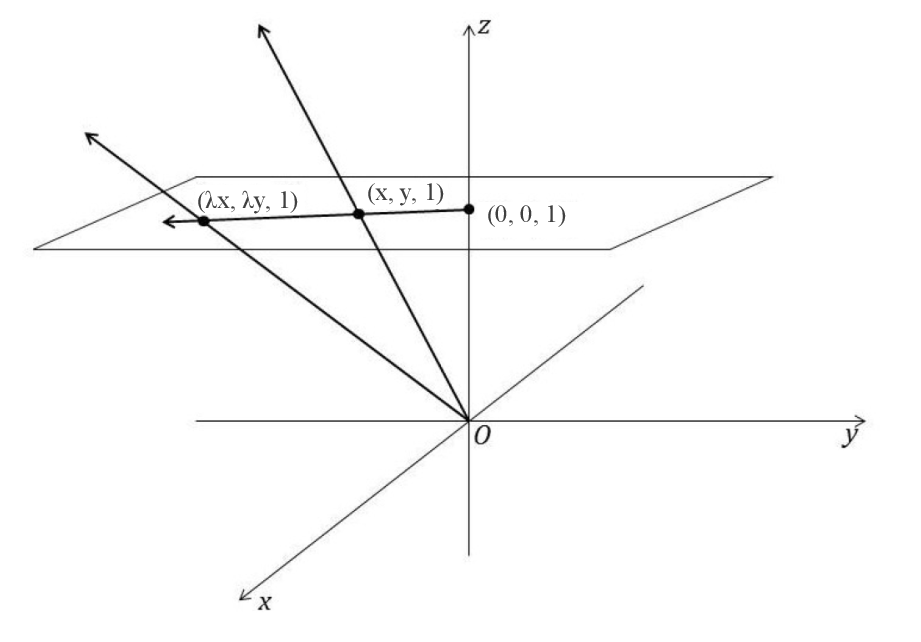
\includegraphics[width=0.8\textwidth]{proGeo_lambda.png}
\caption{die projektive Ebene ${\mathbb{P}}^{2}$ kann als eine eingebettete Ebene im ${\mathbb{R}}^{3}$ verstanden werden \cite{Wahner2011}} 
\label{fig:progeo}
\end{figure} 
Anschaulich werden die Fernpunkte, wenn man eine Ebene betrachtet, die in dem dreidimensionalen Raum ${\mathbb{R}}^{3}$ eingebettet ist. Die Ebene liege parallel zur \textit{xy}-Ebene bei $z = 1$, siehe Abbildung \ref{fig:progeo}. Weiterhin gilt allgemein, dass es f�r jeden Punkt auf der Ebene eine Gerade gibt, die die Ebene schneidet und durch den Ursprung geht. Damit l\"asst sich jedem Punkt der Ebene ein Richtungsvektor zuordnen. Dieser Richtungsvektor kann beispielsweise der Punkt $(x,y,1)$ selbst oder ein skalares Vielfaches von ihm $(\lambda x,\lambda y,1)$, mit $t \in \textbf{R} \setminus \{0\}$, sein. 
Ein beliebiger Punkt auf der Ebene $(\lambda x,\lambda y,1)$ kann ebenfalls als $(x,y,\frac{1}{\lambda})$ geschrieben werden. Man sieht, dass sich der Punkt f�r $\lambda \to \infty$ vom Ursprung entfernt und zu einem Fernpunkt mit $(x,y,0)$ wird. Fernpunkte repr\"asentieren damit die Richtung eines Geradenb�schels\cite{Wahner2011}. Allgemein werden endliche Punkte durch Vektoren der Form $(x,y,1)$ und unendliche Punkte durch $(x,y,0)$ dargestellt.

\subsection {Euklidische und projektive Koordinaten}
Im \textbf{n}-dimensionalen euklidischen Raum ${\mathbb{R}}^{n}$ wird ein Punkt durch einen n-dimensionalen Vektor $\textbf{x} = (x_1,\dots ,x_n)^T$ beschrieben. Diese Darstellung wird auch inhomogene Koordinaten genannt.\\
Ein Punkt im n-dimensionalen projektiven Raum ${\mathbb{P}}^{n}$ wird durch einen \textbf{(n + 1)}-dimensionalen Vektor $\textbf{\~x} = (x_1,\dots ,x_{n+1})^T$ dargestellt. Man spricht in diesem Fall von homogenen Koordinaten. Der Nullvektor $\textbf{0}_{n+1}$ ist kein Element vom ${\mathbb{P}}^{n}$, da er keiner geometrischen Gr\"o{\ss}e im projektiven Raum entspricht. Die \"Uberf\"uhrung von euklidischen Koordinaten in projektive Koordinaten l\"asst sich einfach mit folgender Beziehung durchf\"uhren.
\begin{equation}
	(x_1, \dots, x_n) = \textbf{x}\rightarrow \textsl{\~x}= (\lambda x_1, \dots,\lambda x_n, \lambda) 
\end{equation}
Dabei ist $\lambda$ ein beliebiger Skalierungsfaktor, mit $\lambda \in \textbf{R} \setminus \{0\}$. Durch die Betrachtung der R\"uckkonvertierung wird ersichtlich, warum es notwendig ist die Null auszuschlie{\ss}en.
\begin{equation}
	(x_1,\dots,x_n,x_{n+1}) = \textsl{\~x} \rightarrow \textbf{x} = (\frac{x_1}{x_{n+1}},\dots,\frac{x_n}{x_{n+1}})
\end{equation}
Aus dieser Konvertierung ergibt sich auch, dass die \"Aquivalenz zweier projektiver Punkte die Gleichheit der homogenen Koordinaten, bis auf einen Skalierungsfaktor, bedeutet. Daher spricht man bei homogenen Koordinaten auch von Verh\"altniskoordinaten. Punkte der Form $\textsl{\~x}_{\infty}= (x_1,\dots,x_n,0)^T$ sind Punkte im Unendlichen und werden ideale Punkte genannt. Ideale Punkte k\"onnen offensichtlich nicht in inhomogene Koordinaten \"uberf\"uhrt werden. Damit bildet der euklidische Raum einen Teilraum des projektiven Raums\cite{Rahmann2011}.

\subsection{Transformationen}
Im projektiven Raum sind eine Reihe von Transformationen definiert. Da f\"ur die Kalibrierung die Betrachtung der projektiven Ebene ausreicht, wird nur diese behandelt. Alle behandelten Eigenschaften gelten allerdings auch f\"ur den projektiven Raum. Die Transformationen bilden eine Hierarchie. Die allgemeinste Transformation ist die projektive Transformation, darauf folgt die affine Transformation, die \"ahnliche Transformation und die euklidische Transformation, welche die speziellste Transformation ist. F\"ur jede Gruppe von Transformationen gibt es sogenannte Invarianten\footnote{geometrische Gr\"o�en, die durch die Transformation nicht ver\"andert werden}. Die Anzahl von Invarianten nimmt mit der Spezialisierung der Transformation zu. Dabei ist jede Invariante der Obergruppe auch gleichzeitig eine Invariante jeder abgeleiteten Untergruppe \cite{Rahmann2011}.

\subsubsection{projektive Transformation}

Die projektive Transformation ist die allgemeinste Transformation. Sie bildet Punkte auf Punkte und Linien auf Linien ab. Die Beschreibung der projektiven Transformation ist mit Gleichung \ref{eq:proTrans} m\"oglich.
\begin{equation}
\text{\~{x}' }\thicksim \textbf{H} \text{\~{x}}
\label{eq:proTrans}
\end{equation}
Dabei ist \textbf{H} eine regul\"are $3x3$ Matrix. Weiterhin sei die Gleichung homogen. Die Abbildung wird Homographie genannt. Aus der Eigenschaft der regul\"aren Matrix l\"asst sich die Invertierbarkeit der Transformation ableiten. Da es sich um eine homogene Gleichung handelt, sind alle Matrizen \textbf{H} \"aquivalent, so lange sie sich nur durch einen Skalierungsfaktor unterscheiden. Die einzige Invariante der projektiven Transformation ist das Doppelverh\"altnis: $\frac{|AB||CD|}{|AC||BD|}$, wobei A,B,C und D Punkte auf einer Geraden sind und $|AB|$ der Abstand zwischen zwei Punkten ist. Bei neun Matrixelementen ergeben sich acht Freiheitsgrade, da der Skalierungsfaktor abgezogen werden muss \cite{Rahmann2011}. Die projektive Transformation erlaubt die Abbildung unendlich weit entfernter Punkte auf endlich weit entfernte Punkte.
\subsubsection{euklidische Transformation}
Wie bereits erw\"ahnt, ist die euklidische Transformation(Gleichung \ref{eq:euklidTrafo}) die spezialisierteste Transformation im projektiven Raum. 
\begin{equation}
\text{\~{x}' }\thicksim \textbf{H}_\textbf{S} \text{\~{x}}
 = 
\begin{pmatrix}
\textbf{R} & \textbf{t} \\
\textbf{0}^T & 1 \\
\end{pmatrix}
\text{\~{x}}
\label{eq:euklidTrafo}
\end{equation}
Sie ist durch eine Rotation und eine Translation beschrieben und besitzt als Invarianten L�ngen und Fl�chen\cite{Rahmann2011}. \textbf{R} ist eine  Rotationsmatrix und \textbf{t} der Translationsvektor. F\"ur den ${\mathbb{R}}^{2}$ gilt:
\begin{equation}
\textbf{H}_\textbf{S}
 = 
\begin{pmatrix}
cos(\alpha) & -sin(\alpha) & x \\
sin(\alpha) & cos(\alpha) & y \\
0 & 0  & 1 \\
\end{pmatrix}
\label{eq:Hs}
\end{equation} 

\subsubsection{Inverse Perspective Mapping}\label{sec:IPM}
Unter dem sogenannten \textit{inverse perspective mapping}(IPM) versteht man eine geometrische Transformation, die die Effekte der perspektivischen Projektion umkehrt. Daf\"ur wird das Bild in die Vogelperspektive transformiert. 
\begin{figure}[ht]
\centering
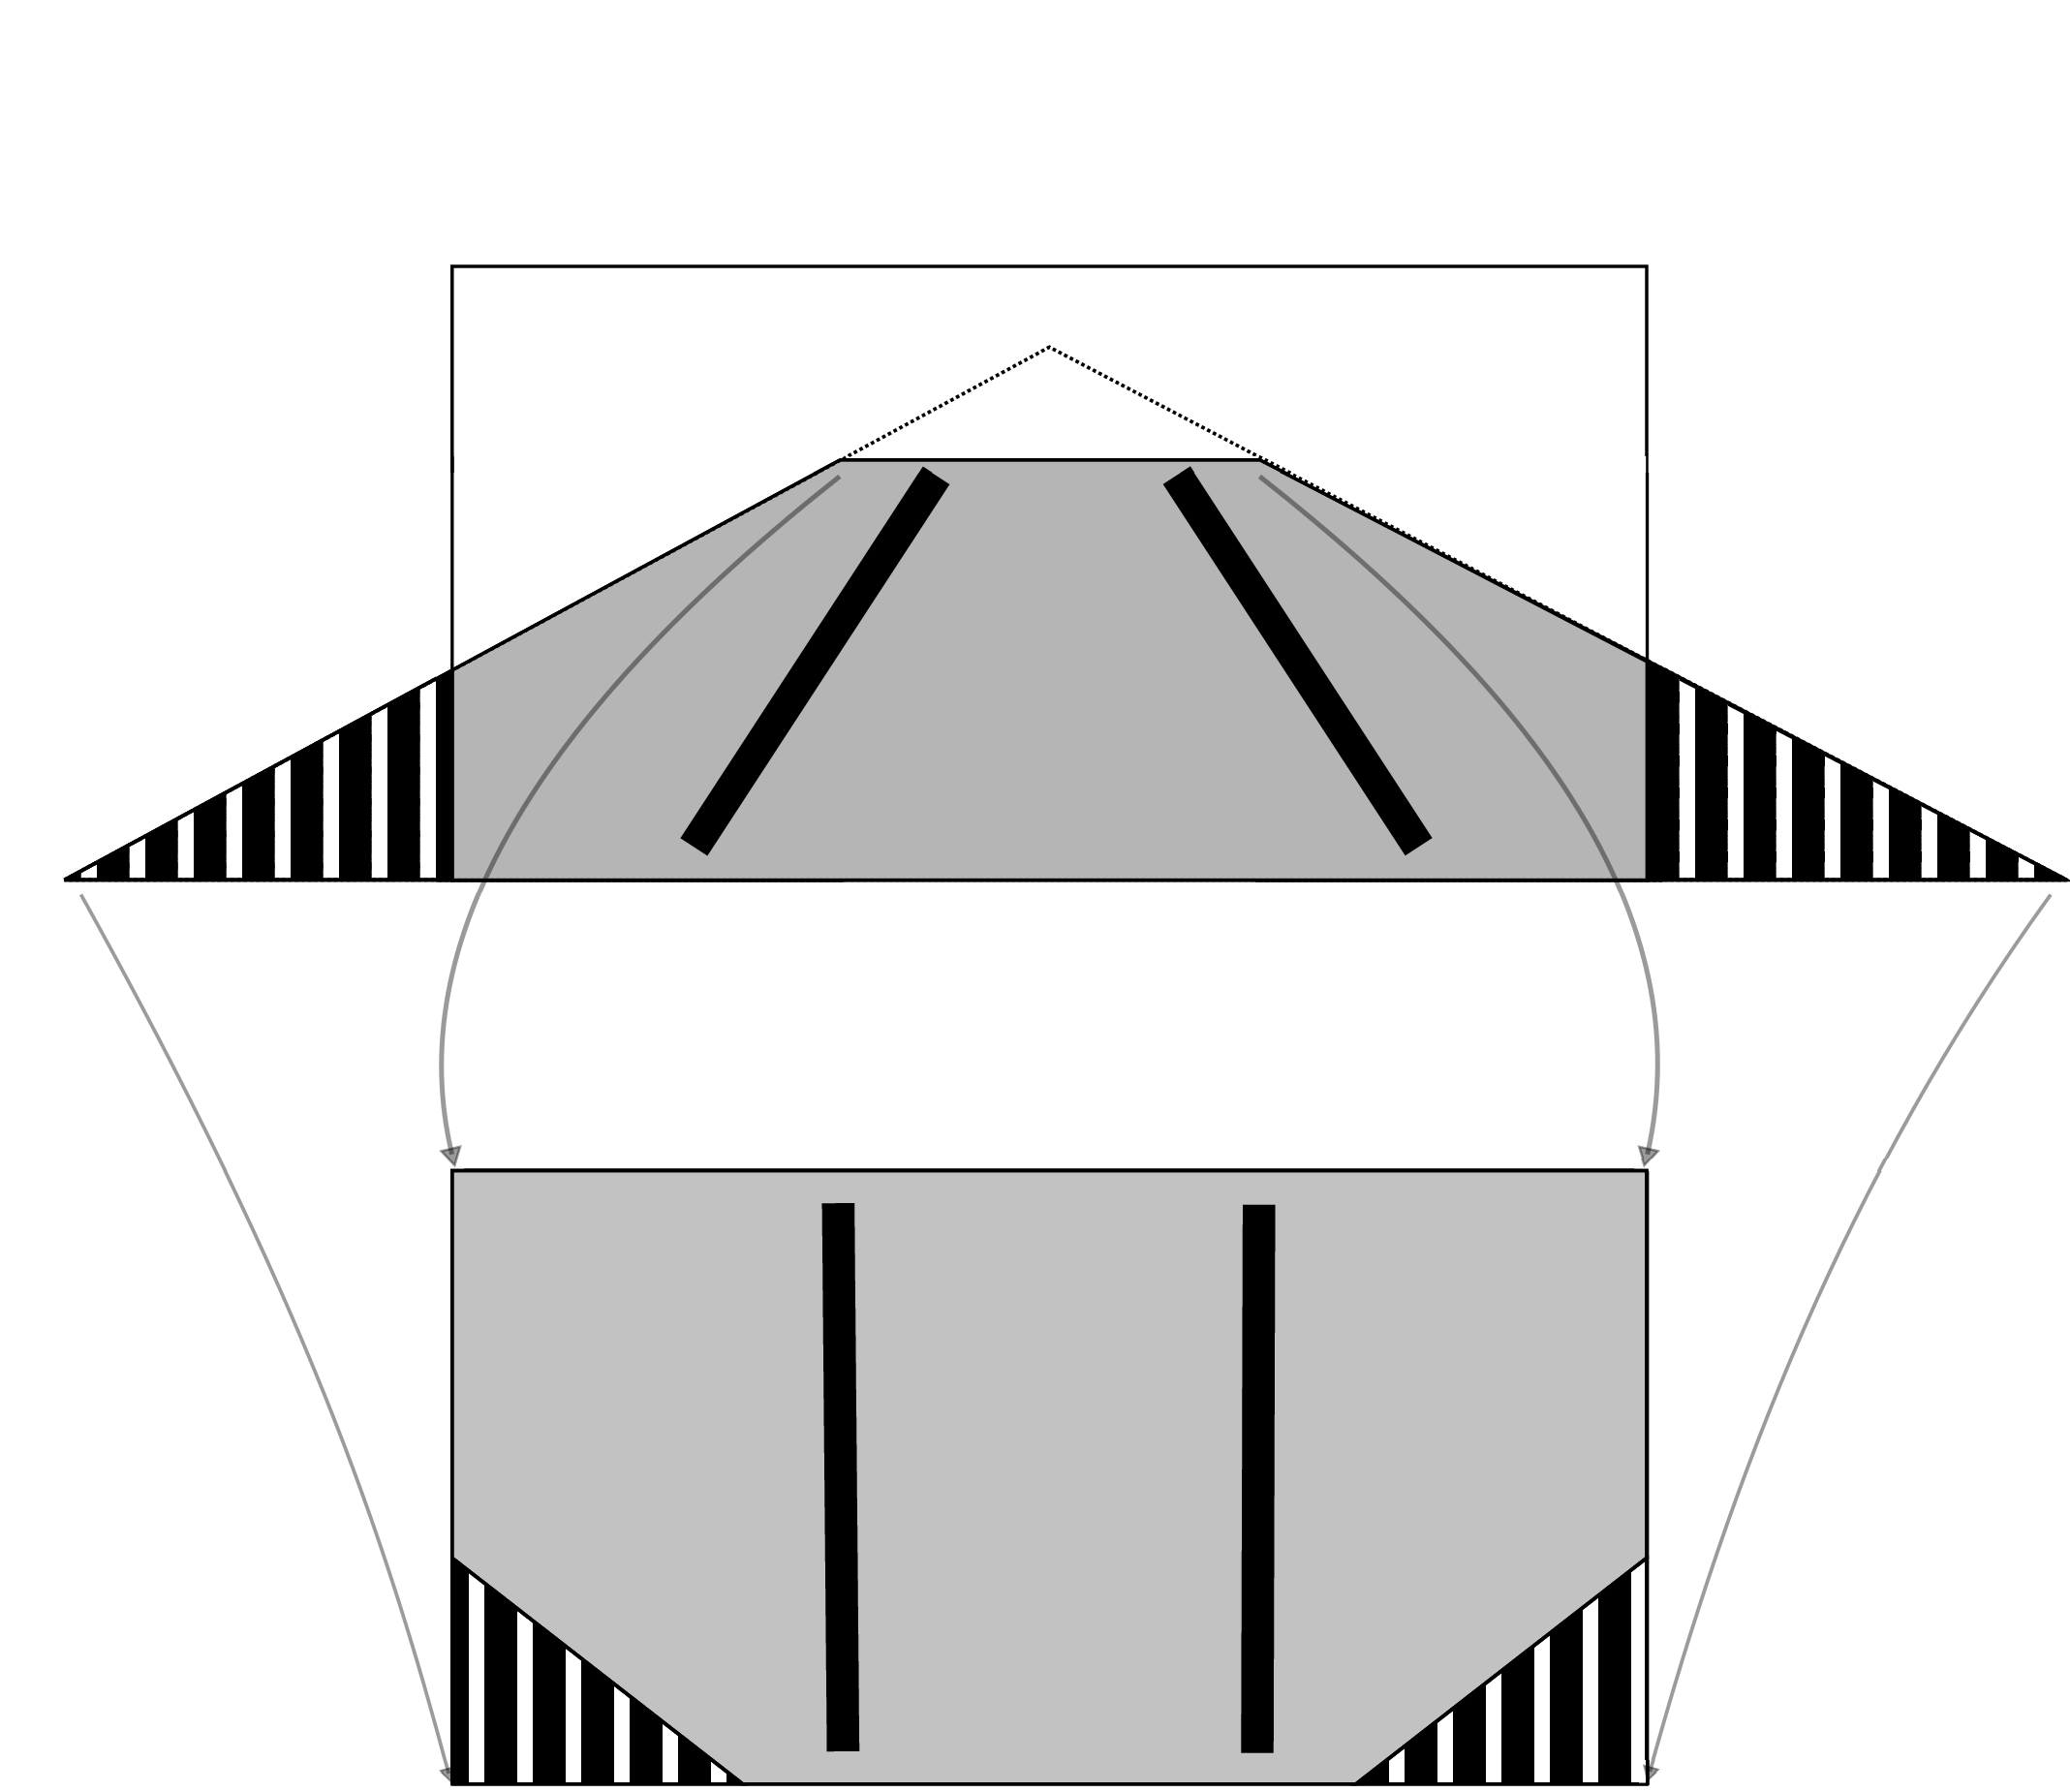
\includegraphics[width=0.8\textwidth]{IPM_Prinzip.png}
\caption{Bei der inversen perspektivischen Transformation werden die Punkte des Ausgangsbildes auf andere Koordinaten abgebildet. Hier dargestellt: die Transformation in die Vogelperspektive} 
\label{fig:IPM_Prinzip}
\end{figure} Abbildung \ref{fig:IPM_Prinzip} zeigt die prinzipielle Funktionsweise der Transformation. Es wird ein Ausschnitt des urspr\"unglichen Bildes auf ein neues Bild abgebildet \cite{AMM2004}. Die Durchf\"uhrung der Transformation ist durch zwei unterschiedliche Verfahren m\"oglich. Die erste berechnet f\"ur jedes Bild eine neue Homographie. Damit ist es beispielsweise m\"oglich, die Transformation auch dann durchzuf\"uhren, wenn die Fahrbahn eine Steigung besitzt. Allerdings ist dieses Verfahren mit hohem Rechenaufwand verbunden. Eine schnellere Methode ist das sogenannte Remapping. Daf\"ur muss im Initialisierungsschritt einmalig eine Punktkorrespondenz gefunden werden, die die Transformation durchf\"uhrt. Mit den Korrespondenzen werden f\"ur das Eingangs- und Ausgangsbild jeweils eine sogenannte \textit{Map} erzeugt. Die \textit{Maps} speichern, auf welche Punkte im Ausgangsbild die Punkte vom Eingangsbild abgebildet werden. Im sp\"ateren Betrieb muss das neue Bild nur einem \textit{remapping} - Schritt unterzogen werden. Dabei werden die Pixel, auf Grundlage der erstellen \textit{Maps}, neu angeordnet. Der Nachteil dieser statischen Methode ist, dass, beispielsweise eine Fahrbahn mit Steigung, nicht korrekt in die Vogelperspektive transformiert wird.

			\chapter{Summary \& Outlook} \label{last_chapter}
\section{Summary}
In this thesis, the time series discretization approaches called \ac{SAX}, \ac{eSAX}, \ac{1d-SAX}, \ac{aSAX}, and Persist were evaluated. \newline
The reconstruction error was used as a metric to quantify and evaluate the goodness of these approaches with respect to a feature-preserving discretized representation of the corresponding original time series. For the reconstruction error, the deviation between the original time series and a numerical reconstruction of the corresponding discretized time series is measured. Qualitatively, the results are as follows:

\textbf{\ac{eSAX} \& \ac{1d-SAX}}: \newline
The \ac{eSAX} and \ac{1d-SAX} perform best across all evaluated time series discretization approaches and configurations. Compared to the other evaluated time series discretization approaches, the \ac{eSAX} and \ac{1d-SAX} benefit from using more information for the discretization of time series.

\textbf{\ac{SAX} \& \ac{aSAX}}: The results for the \ac{SAX} and \ac{aSAX} are similar across all evaluated configurations except for one. For time series with a specific structure, the \ac{aSAX} performs better than the \ac{SAX}. The reason is that the \ac{aSAX} adapts its discretization process to the respective time series at hand, while the \ac{SAX} does not adapt its discretization process.

\textbf{Persist}:
The Persist performs worst across all evaluated time series discretization approaches and configurations, except for the configuration for that the \ac{aSAX} performs better than the \ac{SAX} as explained above. For this configuration, the Persist performs similar to the \ac{aSAX}, as it adapts its discretization process to the time series data at hand, as well.

In addition to measuring the reconstruction error, three motif discovery algorithms were applied to evaluate the applicability of the examined time series discretization approaches as a preprocessing step for those motif discovery algorithms. Qualitatively, the \ac{SAX}, \ac{aSAX}, and Persist perform similar across all evaluated configurations, while the \ac{eSAX} performs worst. Moreover, the results indicate that the \ac{1d-SAX} slightly outperforms all other evaluated time series discretization approaches for one of the three applied motif discovery algorithms. For the other two, the \ac{1d-SAX} performs similar to the \ac{SAX}, \ac{aSAX}, and Persist. \newline
For comparison, two of the three applied motif discovery algorithms were also executed with the original time series as input (i.e. without any preprocessing step). Overall, these results indicate that the precision with which recurrently occurring patterns in time series are detected only decreases slightly, if at all, when using the time series discretization algorithms for preprocessing. However, the number of recurrently occurring patterns detected in time series decreases more and more often.
\section{Outlook}
In this thesis, a time series is assumed to be univariate, meaning that for each observed point in time, there is only one observation \cite{Survey_Esling}. However, time series can also be multivariate, meaning that for each observed point in time there are multiple, but the same number of observations, where each observation belongs to a different univariate time series \cite{Survey_Esling}. Therefore, a possible extension of the evaluation in this thesis, could comprise time series discretization approaches that are applicable for multivariate time series. \newline
Moreover, in this thesis, it is assumed that the observations of a time series are observed at uniformly spaced points in time. This assumption could be relaxed by evaluating time series discretization approaches that are applicable for time series with observations that are observed at irregularly spaced points in time. \newline
Lastly, this thesis focuses on motif discovery with respect to time series pattern recognition. This scope could be extended by incorporating other tasks of time series pattern recognition like anomaly detection \cite{Survey_Esling}. 
 
			\chapter{Summary \& Outlook} \label{last_chapter}
\section{Summary}
In this thesis, the time series discretization approaches called \ac{SAX}, \ac{eSAX}, \ac{1d-SAX}, \ac{aSAX}, and Persist were evaluated. \newline
The reconstruction error was used as a metric to quantify and evaluate the goodness of these approaches with respect to a feature-preserving discretized representation of the corresponding original time series. For the reconstruction error, the deviation between the original time series and a numerical reconstruction of the corresponding discretized time series is measured. Qualitatively, the results are as follows:

\textbf{\ac{eSAX} \& \ac{1d-SAX}}: \newline
The \ac{eSAX} and \ac{1d-SAX} perform best across all evaluated time series discretization approaches and configurations. Compared to the other evaluated time series discretization approaches, the \ac{eSAX} and \ac{1d-SAX} benefit from using more information for the discretization of time series.

\textbf{\ac{SAX} \& \ac{aSAX}}: The results for the \ac{SAX} and \ac{aSAX} are similar across all evaluated configurations except for one. For time series with a specific structure, the \ac{aSAX} performs better than the \ac{SAX}. The reason is that the \ac{aSAX} adapts its discretization process to the respective time series at hand, while the \ac{SAX} does not adapt its discretization process.

\textbf{Persist}:
The Persist performs worst across all evaluated time series discretization approaches and configurations, except for the configuration for that the \ac{aSAX} performs better than the \ac{SAX} as explained above. For this configuration, the Persist performs similar to the \ac{aSAX}, as it adapts its discretization process to the time series data at hand, as well.

In addition to measuring the reconstruction error, three motif discovery algorithms were applied to evaluate the applicability of the examined time series discretization approaches as a preprocessing step for those motif discovery algorithms. Qualitatively, the \ac{SAX}, \ac{aSAX}, and Persist perform similar across all evaluated configurations, while the \ac{eSAX} performs worst. Moreover, the results indicate that the \ac{1d-SAX} slightly outperforms all other evaluated time series discretization approaches for one of the three applied motif discovery algorithms. For the other two, the \ac{1d-SAX} performs similar to the \ac{SAX}, \ac{aSAX}, and Persist. \newline
For comparison, two of the three applied motif discovery algorithms were also executed with the original time series as input (i.e. without any preprocessing step). Overall, these results indicate that the precision with which recurrently occurring patterns in time series are detected only decreases slightly, if at all, when using the time series discretization algorithms for preprocessing. However, the number of recurrently occurring patterns detected in time series decreases more and more often.
\section{Outlook}
In this thesis, a time series is assumed to be univariate, meaning that for each observed point in time, there is only one observation \cite{Survey_Esling}. However, time series can also be multivariate, meaning that for each observed point in time there are multiple, but the same number of observations, where each observation belongs to a different univariate time series \cite{Survey_Esling}. Therefore, a possible extension of the evaluation in this thesis, could comprise time series discretization approaches that are applicable for multivariate time series. \newline
Moreover, in this thesis, it is assumed that the observations of a time series are observed at uniformly spaced points in time. This assumption could be relaxed by evaluating time series discretization approaches that are applicable for time series with observations that are observed at irregularly spaced points in time. \newline
Lastly, this thesis focuses on motif discovery with respect to time series pattern recognition. This scope could be extended by incorporating other tasks of time series pattern recognition like anomaly detection \cite{Survey_Esling}. 
 			
			\chapter{Summary \& Outlook} \label{last_chapter}
\section{Summary}
In this thesis, the time series discretization approaches called \ac{SAX}, \ac{eSAX}, \ac{1d-SAX}, \ac{aSAX}, and Persist were evaluated. \newline
The reconstruction error was used as a metric to quantify and evaluate the goodness of these approaches with respect to a feature-preserving discretized representation of the corresponding original time series. For the reconstruction error, the deviation between the original time series and a numerical reconstruction of the corresponding discretized time series is measured. Qualitatively, the results are as follows:

\textbf{\ac{eSAX} \& \ac{1d-SAX}}: \newline
The \ac{eSAX} and \ac{1d-SAX} perform best across all evaluated time series discretization approaches and configurations. Compared to the other evaluated time series discretization approaches, the \ac{eSAX} and \ac{1d-SAX} benefit from using more information for the discretization of time series.

\textbf{\ac{SAX} \& \ac{aSAX}}: The results for the \ac{SAX} and \ac{aSAX} are similar across all evaluated configurations except for one. For time series with a specific structure, the \ac{aSAX} performs better than the \ac{SAX}. The reason is that the \ac{aSAX} adapts its discretization process to the respective time series at hand, while the \ac{SAX} does not adapt its discretization process.

\textbf{Persist}:
The Persist performs worst across all evaluated time series discretization approaches and configurations, except for the configuration for that the \ac{aSAX} performs better than the \ac{SAX} as explained above. For this configuration, the Persist performs similar to the \ac{aSAX}, as it adapts its discretization process to the time series data at hand, as well.

In addition to measuring the reconstruction error, three motif discovery algorithms were applied to evaluate the applicability of the examined time series discretization approaches as a preprocessing step for those motif discovery algorithms. Qualitatively, the \ac{SAX}, \ac{aSAX}, and Persist perform similar across all evaluated configurations, while the \ac{eSAX} performs worst. Moreover, the results indicate that the \ac{1d-SAX} slightly outperforms all other evaluated time series discretization approaches for one of the three applied motif discovery algorithms. For the other two, the \ac{1d-SAX} performs similar to the \ac{SAX}, \ac{aSAX}, and Persist. \newline
For comparison, two of the three applied motif discovery algorithms were also executed with the original time series as input (i.e. without any preprocessing step). Overall, these results indicate that the precision with which recurrently occurring patterns in time series are detected only decreases slightly, if at all, when using the time series discretization algorithms for preprocessing. However, the number of recurrently occurring patterns detected in time series decreases more and more often.
\section{Outlook}
In this thesis, a time series is assumed to be univariate, meaning that for each observed point in time, there is only one observation \cite{Survey_Esling}. However, time series can also be multivariate, meaning that for each observed point in time there are multiple, but the same number of observations, where each observation belongs to a different univariate time series \cite{Survey_Esling}. Therefore, a possible extension of the evaluation in this thesis, could comprise time series discretization approaches that are applicable for multivariate time series. \newline
Moreover, in this thesis, it is assumed that the observations of a time series are observed at uniformly spaced points in time. This assumption could be relaxed by evaluating time series discretization approaches that are applicable for time series with observations that are observed at irregularly spaced points in time. \newline
Lastly, this thesis focuses on motif discovery with respect to time series pattern recognition. This scope could be extended by incorporating other tasks of time series pattern recognition like anomaly detection \cite{Survey_Esling}. 
 
			\chapter{Summary \& Outlook} \label{last_chapter}
\section{Summary}
In this thesis, the time series discretization approaches called \ac{SAX}, \ac{eSAX}, \ac{1d-SAX}, \ac{aSAX}, and Persist were evaluated. \newline
The reconstruction error was used as a metric to quantify and evaluate the goodness of these approaches with respect to a feature-preserving discretized representation of the corresponding original time series. For the reconstruction error, the deviation between the original time series and a numerical reconstruction of the corresponding discretized time series is measured. Qualitatively, the results are as follows:

\textbf{\ac{eSAX} \& \ac{1d-SAX}}: \newline
The \ac{eSAX} and \ac{1d-SAX} perform best across all evaluated time series discretization approaches and configurations. Compared to the other evaluated time series discretization approaches, the \ac{eSAX} and \ac{1d-SAX} benefit from using more information for the discretization of time series.

\textbf{\ac{SAX} \& \ac{aSAX}}: The results for the \ac{SAX} and \ac{aSAX} are similar across all evaluated configurations except for one. For time series with a specific structure, the \ac{aSAX} performs better than the \ac{SAX}. The reason is that the \ac{aSAX} adapts its discretization process to the respective time series at hand, while the \ac{SAX} does not adapt its discretization process.

\textbf{Persist}:
The Persist performs worst across all evaluated time series discretization approaches and configurations, except for the configuration for that the \ac{aSAX} performs better than the \ac{SAX} as explained above. For this configuration, the Persist performs similar to the \ac{aSAX}, as it adapts its discretization process to the time series data at hand, as well.

In addition to measuring the reconstruction error, three motif discovery algorithms were applied to evaluate the applicability of the examined time series discretization approaches as a preprocessing step for those motif discovery algorithms. Qualitatively, the \ac{SAX}, \ac{aSAX}, and Persist perform similar across all evaluated configurations, while the \ac{eSAX} performs worst. Moreover, the results indicate that the \ac{1d-SAX} slightly outperforms all other evaluated time series discretization approaches for one of the three applied motif discovery algorithms. For the other two, the \ac{1d-SAX} performs similar to the \ac{SAX}, \ac{aSAX}, and Persist. \newline
For comparison, two of the three applied motif discovery algorithms were also executed with the original time series as input (i.e. without any preprocessing step). Overall, these results indicate that the precision with which recurrently occurring patterns in time series are detected only decreases slightly, if at all, when using the time series discretization algorithms for preprocessing. However, the number of recurrently occurring patterns detected in time series decreases more and more often.
\section{Outlook}
In this thesis, a time series is assumed to be univariate, meaning that for each observed point in time, there is only one observation \cite{Survey_Esling}. However, time series can also be multivariate, meaning that for each observed point in time there are multiple, but the same number of observations, where each observation belongs to a different univariate time series \cite{Survey_Esling}. Therefore, a possible extension of the evaluation in this thesis, could comprise time series discretization approaches that are applicable for multivariate time series. \newline
Moreover, in this thesis, it is assumed that the observations of a time series are observed at uniformly spaced points in time. This assumption could be relaxed by evaluating time series discretization approaches that are applicable for time series with observations that are observed at irregularly spaced points in time. \newline
Lastly, this thesis focuses on motif discovery with respect to time series pattern recognition. This scope could be extended by incorporating other tasks of time series pattern recognition like anomaly detection \cite{Survey_Esling}. 
 
			\chapter{Summary \& Outlook} \label{last_chapter}
\section{Summary}
In this thesis, the time series discretization approaches called \ac{SAX}, \ac{eSAX}, \ac{1d-SAX}, \ac{aSAX}, and Persist were evaluated. \newline
The reconstruction error was used as a metric to quantify and evaluate the goodness of these approaches with respect to a feature-preserving discretized representation of the corresponding original time series. For the reconstruction error, the deviation between the original time series and a numerical reconstruction of the corresponding discretized time series is measured. Qualitatively, the results are as follows:

\textbf{\ac{eSAX} \& \ac{1d-SAX}}: \newline
The \ac{eSAX} and \ac{1d-SAX} perform best across all evaluated time series discretization approaches and configurations. Compared to the other evaluated time series discretization approaches, the \ac{eSAX} and \ac{1d-SAX} benefit from using more information for the discretization of time series.

\textbf{\ac{SAX} \& \ac{aSAX}}: The results for the \ac{SAX} and \ac{aSAX} are similar across all evaluated configurations except for one. For time series with a specific structure, the \ac{aSAX} performs better than the \ac{SAX}. The reason is that the \ac{aSAX} adapts its discretization process to the respective time series at hand, while the \ac{SAX} does not adapt its discretization process.

\textbf{Persist}:
The Persist performs worst across all evaluated time series discretization approaches and configurations, except for the configuration for that the \ac{aSAX} performs better than the \ac{SAX} as explained above. For this configuration, the Persist performs similar to the \ac{aSAX}, as it adapts its discretization process to the time series data at hand, as well.

In addition to measuring the reconstruction error, three motif discovery algorithms were applied to evaluate the applicability of the examined time series discretization approaches as a preprocessing step for those motif discovery algorithms. Qualitatively, the \ac{SAX}, \ac{aSAX}, and Persist perform similar across all evaluated configurations, while the \ac{eSAX} performs worst. Moreover, the results indicate that the \ac{1d-SAX} slightly outperforms all other evaluated time series discretization approaches for one of the three applied motif discovery algorithms. For the other two, the \ac{1d-SAX} performs similar to the \ac{SAX}, \ac{aSAX}, and Persist. \newline
For comparison, two of the three applied motif discovery algorithms were also executed with the original time series as input (i.e. without any preprocessing step). Overall, these results indicate that the precision with which recurrently occurring patterns in time series are detected only decreases slightly, if at all, when using the time series discretization algorithms for preprocessing. However, the number of recurrently occurring patterns detected in time series decreases more and more often.
\section{Outlook}
In this thesis, a time series is assumed to be univariate, meaning that for each observed point in time, there is only one observation \cite{Survey_Esling}. However, time series can also be multivariate, meaning that for each observed point in time there are multiple, but the same number of observations, where each observation belongs to a different univariate time series \cite{Survey_Esling}. Therefore, a possible extension of the evaluation in this thesis, could comprise time series discretization approaches that are applicable for multivariate time series. \newline
Moreover, in this thesis, it is assumed that the observations of a time series are observed at uniformly spaced points in time. This assumption could be relaxed by evaluating time series discretization approaches that are applicable for time series with observations that are observed at irregularly spaced points in time. \newline
Lastly, this thesis focuses on motif discovery with respect to time series pattern recognition. This scope could be extended by incorporating other tasks of time series pattern recognition like anomaly detection \cite{Survey_Esling}. 
 
			\chapter{Summary \& Outlook} \label{last_chapter}
\section{Summary}
In this thesis, the time series discretization approaches called \ac{SAX}, \ac{eSAX}, \ac{1d-SAX}, \ac{aSAX}, and Persist were evaluated. \newline
The reconstruction error was used as a metric to quantify and evaluate the goodness of these approaches with respect to a feature-preserving discretized representation of the corresponding original time series. For the reconstruction error, the deviation between the original time series and a numerical reconstruction of the corresponding discretized time series is measured. Qualitatively, the results are as follows:

\textbf{\ac{eSAX} \& \ac{1d-SAX}}: \newline
The \ac{eSAX} and \ac{1d-SAX} perform best across all evaluated time series discretization approaches and configurations. Compared to the other evaluated time series discretization approaches, the \ac{eSAX} and \ac{1d-SAX} benefit from using more information for the discretization of time series.

\textbf{\ac{SAX} \& \ac{aSAX}}: The results for the \ac{SAX} and \ac{aSAX} are similar across all evaluated configurations except for one. For time series with a specific structure, the \ac{aSAX} performs better than the \ac{SAX}. The reason is that the \ac{aSAX} adapts its discretization process to the respective time series at hand, while the \ac{SAX} does not adapt its discretization process.

\textbf{Persist}:
The Persist performs worst across all evaluated time series discretization approaches and configurations, except for the configuration for that the \ac{aSAX} performs better than the \ac{SAX} as explained above. For this configuration, the Persist performs similar to the \ac{aSAX}, as it adapts its discretization process to the time series data at hand, as well.

In addition to measuring the reconstruction error, three motif discovery algorithms were applied to evaluate the applicability of the examined time series discretization approaches as a preprocessing step for those motif discovery algorithms. Qualitatively, the \ac{SAX}, \ac{aSAX}, and Persist perform similar across all evaluated configurations, while the \ac{eSAX} performs worst. Moreover, the results indicate that the \ac{1d-SAX} slightly outperforms all other evaluated time series discretization approaches for one of the three applied motif discovery algorithms. For the other two, the \ac{1d-SAX} performs similar to the \ac{SAX}, \ac{aSAX}, and Persist. \newline
For comparison, two of the three applied motif discovery algorithms were also executed with the original time series as input (i.e. without any preprocessing step). Overall, these results indicate that the precision with which recurrently occurring patterns in time series are detected only decreases slightly, if at all, when using the time series discretization algorithms for preprocessing. However, the number of recurrently occurring patterns detected in time series decreases more and more often.
\section{Outlook}
In this thesis, a time series is assumed to be univariate, meaning that for each observed point in time, there is only one observation \cite{Survey_Esling}. However, time series can also be multivariate, meaning that for each observed point in time there are multiple, but the same number of observations, where each observation belongs to a different univariate time series \cite{Survey_Esling}. Therefore, a possible extension of the evaluation in this thesis, could comprise time series discretization approaches that are applicable for multivariate time series. \newline
Moreover, in this thesis, it is assumed that the observations of a time series are observed at uniformly spaced points in time. This assumption could be relaxed by evaluating time series discretization approaches that are applicable for time series with observations that are observed at irregularly spaced points in time. \newline
Lastly, this thesis focuses on motif discovery with respect to time series pattern recognition. This scope could be extended by incorporating other tasks of time series pattern recognition like anomaly detection \cite{Survey_Esling}. 
 
\printbibliography

\end{document}